%%%%%%%%%%%%%%%%%%%%%%%%%%%%%%%%%%%%%%%%%%%%%%%%%%%%%%%%%%%%%%%%%%%%%%
% LaTeX Template: Curriculum Vitae
%
% Source: http://www.howtotex.com/
% Feel free to distribute this template, but please keep the
% referal to HowToTeX.com.
% Date: July 2011
%Version for spanish users, by dgarhdez
% 
%%%%%%%%%%%%%%%%%%%%%%%%%%%%%%%%%%%%%%%%%%%%%%%%%%%%%%%%%%%%%%%%%%%%%%
% How to use writeLaTeX: 
%
% You edit the source code here on the left, and the preview on the
% right shows you the result within a few seconds.
%
% Bookmark this page and share the URL with your co-authors. They can
% edit at the same time!
%
% You can upload figures, bibliographies, custom classes and
% styles using the files menu.
%
% If you're new to LaTeX, the wikibook is a great place to start:
% http://en.wikibooks.org/wiki/LaTeX
%
%%%%%%%%%%%%%%%%%%%%%%%%%%%%%%%%%%%%%%%%%%%%%%%%%%%%%%%%%%%%%%%%%%%%%%
\documentclass[paper=a4,fontsize=11pt]{scrartcl} % KOMA-article class
\usepackage[protrusion=true,expansion=true]{microtype}
\usepackage{amsmath,amsfonts,amsthm}     % Math packages
\usepackage{graphicx}                    % Enable pdflatex
\usepackage[svgnames]{xcolor}            % Colors by their 'svgnames'
\usepackage{geometry}
	\textheight=700px                    % Saving trees ;-)
\usepackage{url}
\usepackage{CJKutf8}
\frenchspacing              % Better looking spacings after periods
\pagestyle{empty}           % No pagenumbers/headers/footers

%%% Custom sectioning (sectsty package)
%%% ------------------------------------------------------------
\usepackage{sectsty}

\sectionfont{%			            % Change font of \section command
	\usefont{OT1}{phv}{b}{n}%		% bch-b-n: CharterBT-Bold font
	\sectionrule{0pt}{0pt}{-5pt}{1pt}}

%%% Macros
%%% ------------------------------------------------------------
\newlength{\spacebox}
\settowidth{\spacebox}{8888888888}			% Box to align text
\newcommand{\sepspace}{\vspace*{1em}}		% Vertical space macro

\newcommand{\MyName}[1]{ % Name
		\Huge \usefont{OT1}{phv}{b}{n} \hfill #1
		\par \normalsize \normalfont}
		
\newcommand{\MySlogan}[1]{ % Slogan (optional)
		\large \usefont{OT1}{phv}{m}{n}\hfill \textit{#1}
		\par \normalsize \normalfont}

\newcommand{\NewPart}[1]{\section*{\uppercase{#1}}}

\newcommand{\PersonalEntry}[2]{
		\noindent\hangindent=2em\hangafter=0 % Indentation
		\parbox{\spacebox}{        % Box to align text
		\textit{#1}}		       % Entry name (birth, address, etc.)
		\hspace{1.5em} #2 \par}    % Entry value

\newcommand{\SkillsEntry}[2]{      % Same as \PersonalEntry
		\noindent\hangindent=2em\hangafter=0 % Indentation
		\parbox{\spacebox}{        % Box to align text
		\textit{#1}}			   % Entry name (birth, address, etc.)
		\hspace{1.5em} #2 \par}    % Entry value	
		
\newcommand{\EducationEntry}[4]{
		\noindent \textbf{#1} \hfill      % Study
		\colorbox{White}{%
			\parbox{5cm}{%
			\hfill\color{Black}#2}} \par  % Duration
		\noindent \textit{#3} \par        % School
		\noindent\hangindent=2em\hangafter=0 \small #4 % Description
		\normalsize \par}

\newcommand{\WorkEntry}[4]{				  % Same as \EducationEntry
		\noindent \textbf{#1} \hfill      % Jobname
		\noindent\colorbox{Black}{\color{White}#2} \par  % Duration
		\noindent \textit{#3} \par              % Company
		\noindent\hangindent=2em\hangafter=0 \small #4 % Description
		\normalsize \par}

%%% Begin Document
%%% ------------------------------------------------------------
\begin{document}
		\begin{CJK*}{UTF8}{gbsn}
% you can upload a photo and include it here...
%\begin{wrapfigure}{l}{0.5\textwidth}
%	\vspace*{-2em}
%		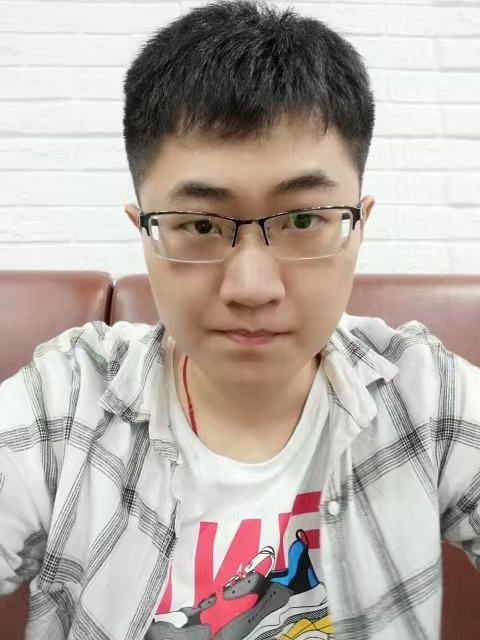
\includegraphics[width=0.15\textwidth]{photo}
%\end{wrapfigure}
{\centering{ \Huge \usefont{OT1}{phv}{b}{n} {杜旭}}
	\par \normalsize \normalfont}
%\MyName{Xu Du}
%\MySlogan{Nombre de tu carrera}

%\sepspace

%%% Personal details
%%% ------------------------------------------------------------
\NewPart{联系方式}{}

\PersonalEntry{地址:}{ 西源大道2006号, 成都, 中国}
%\PersonalEntry{Address}{111 First St, New York}
\PersonalEntry{主页:}{https://fubianhanshu9.github.io/index.html}
\PersonalEntry{邮箱:}{\url{duxu@uestc.edu.cn}}%{\url{duxu@shanghaitech.edu.cn}}

%%% Education
%%% ------------------------------------------------------------
%\NewPart{工作经历}
%\begin{itemize}
%	\item 博士后研究员, 电子科技大学通信抗干扰国家重点实验室  (合作导师:袁晓军教授), 2023-现在.
%\end{itemize}

%\textbf{Boris Houska}
\NewPart{教育经历}{}

\EducationEntry{中国科学院大学\\中国科学院上海微系统与信息技术研究所}{2017.9-2022.9}{通信与信息系统工学博士 ( 导师:Boris Houska 教授) }
%{\begin{itemize}
%\item{Especialidad }
%\item{Asignaturas más relevantes de carrera/especialidad}
%\item{Proyecto de fin de carrera: \emph{título del proyecto}}
%\end{itemize}
%}

\sepspace

\EducationEntry{郑州大学,信息工程学院}{2013.9-2017.7}{计算机科学与技术工学学士 }

%%% Work experience
%%% ------------------------------------------------------------
\NewPart{研究兴趣}{}
%\EducationEntry{Power System State Estimation}
\begin{itemize}
	\item{最优实验设计}
	
	\item{分布式数值优化}
	
	\item{电力系统}
%	\item{Algorithmic Game Theory}
	\item{无线通信}
	\item{算法博弈论}
		\item{鲁棒优化}
\end{itemize}


\NewPart{出版物}{}
$\dag$:  共同一作
%\textbf{Conference Paper}
%\EducationEntry{Power System State Estimation}
%\section{Conference}
\begin{itemize}
		\item  { \textbf{Xu Du}$^{\dag}$, Shijie Zhu$^{\dag}$, Yifei Wang$^{\dag}$, Boyu Han$^{\dag}$, Xiaohe He$^{\dag}$. \\
		{Optimal Resilience Design of AC Microgrid
			using AO-SBQP Method}\\
		\emph{ The 22nd IFAC World Congress, Yokohama, Japan, 2023  已接收	} }
	
	
		\item  { \textbf{Xu Du}, Alexander Engelmann, Timm Faulwasser, Boris Houska. \\
		{Approximations for Optimal Experimental Design
			in Power System Parameter Estimation (invited session)}\\
		\emph{ The 61th IEEE Conference on Decision and Control (CDC), Canc\'un, Mexico, 2022
		} }
	
	
	\item  { Shijie Zhu$^{\dag}$, \textbf{Xu Du}$^{\dag}$. \\
		{Alternating Direction Based Sequential Boolean Quadratic Programming Method for Transmit Antenna Selection}\\
		\emph{ The 61th IEEE Conference on Decision and Control (CDC), Canc\'un, Mexico, 2022
	} }
	
		\item  { Boyu Han, Xuwen Liang, Zhuochen Xie, \textbf{Xu Du}, Xiaohe He. \\
		{Communication Enhancement Model of Intelligent Reflecting Surface Based on Cooperative Relationship}\\
		\emph{Laser $\&$ Optoelectronics Progress, 2021
	} }
	
	\item  { \textbf{Xu Du}, Alexander Engelmann, Timm Faulwasser, Boris Houska. \\
		{Online power system parameter estimation and optimal operation}\\
		\emph{In Proceedings of the 2021 American Control Conference (ACC), New Orleans, USA May, 2021
	} }
	
		\item  {\textbf{Xu Du}, Alexander Engelmann, Yuning Jiang, Timm Faulwasser, Boris Houska. \\
		Optimal Experiment Design for AC Power Systems Admittance Estimation\\
		\emph{In Proceedings of the 21rst IFAC World Congress, Berlin, Germany, July, 2020
		} }
	
	\item  {\textbf{Xu Du}, Alexander Engelmann, Yuning Jiang, Timm Faulwasser, Boris Houska. \\
		Distributed State Estimation for AC Power Systems using Gauss-Newton ALADIN \\
		 \emph{In Proceedings of the 58th IEEE Conference on Decision and Control (CDC),
		Nice, France, December, 2019.} }
	%\item{Optimal Experimental Design}
	%\item{Función 3}
\end{itemize}
%\textbf{Journal Article }
%\section{Journal}
注:IEEE CDC, IEEE ACC与IFAC World Congress为控制领域三大顶级会议,其中IFAC World Congress第一年于1960年召开,之后每三年召开一次。
\NewPart{学术服务}{会议共同主席/参与主办}
%
%\EducationEntry{Título trabajo 1}{Periodo}{Empresa}{
\begin{itemize}
	\item{邀请会议The 61st
		IEEE Conference on Decision and Control (CDC 2022)
		“Trends in Optimization for Power Systems”, Canc\'un, Mexico联合主席}
	\end{itemize}
{学术会议举办}
\begin{itemize}
\item{International Workshop on Advanced Methods for Control and Estimation of Dynamic
	Systems (AMCEDS 2018), ShanghaiTech University, Shanghai, China, July 23, 2018}
%\item{Función 2}
%\item{Función 3}
\end{itemize}
{论文审稿}
\begin{itemize}
	\item 期刊: Optimal Control Applications $\&$ Methods
	\item 会议: IEEE CDC, IFAC World Congress,IEEE ICCA
\end{itemize}

\NewPart{学术演讲}{}
\begin{itemize}
	
	\item {
		{Sublinear Convergence of ADMM}\\
		\emph{上海科技大学, 上海, 2022年12月8日 (线上)	} }
	\item  {
		{Distributed Optimization with ADMM and ALADIN}\\
		\emph{中国科学院微小卫星创新研究院, 上海, 2021年11月
	} }
	
	
	\item  {
		{Online power system parameter estimation and optimal operation}\\
		\emph{2021 American Control Conference (ACC), 美国新奥尔良, 2021年5月 (线上)
	} }
	
	\item  {
		Optimal Experiment Design for AC Power Systems Admittance Estimation\\
		\emph{21rst IFAC World Congress, 德国柏林, 2020年7月 (线上)
	} }
	
	\item  {
		Distributed State Estimation for AC Power Systems using Gauss-Newton ALADIN 
		\emph{58th IEEE Conference on Decision and Control (CDC),
			法国尼斯, 2019年12月} }
\end{itemize}


\NewPart{获奖与荣誉}
\begin{itemize}
	\item 优秀学生, 上海科技大学, 2019-2020
	
	\item 信息学院优秀助教, 上海科技大学, 2019-2020
		
	%\item SIST Outstanding Teaching Assistant Award, ShanghaiTech University, 2019
	
	\item 优秀学生, 郑州大学, 2014-2017
	
	\item 易盛奖学金, 郑州大学, 2015
	
	
	\end{itemize}
%\sepspace
%
%\EducationEntry{Título trabajo 2}{Periodo}{Empresa}{Descripción, habilidades}
\NewPart{URL 链接}
\begin{itemize}
	\item 谷歌学术: \url{https://scholar.google.com/citations?user=OnIuCR0AAAAJ}
	\item ResearchGate: \url{https://www.researchgate.net/profile/Xu-Du-9}
\end{itemize}
\NewPart{学生指导}{联合指导}
\begin{itemize}
	\item 韩博宇, 中国科学院微小卫星创新研究院, 2021。\\
	(2021年硕士学位 , 任职于中国银联)
	\item 朱时捷, 中国科学院微小卫星创新研究院, 2021-2023。\\
	(2023年硕士学位)
	\item 王逸飞, 中国科学院微小卫星创新研究院, 2021-2023。\\
	(2023年硕士学位)
\end{itemize}

\NewPart{教学}{上海科技大学}
\begin{itemize}
	
	
	\item{助教, 	通信原理(EE140), 上海科技大学, 2021秋季 (廉黎祥教授)}
	
	\item{助教,  信号与系统实验(EE150L), 上海科技大学, 2021春季 (陆林燕,王萍)}
	
	\item{助教, 控制原理(EE160), 上海科技大学, 2020秋季\\ 
		http://faculty.sist.shanghaitech.edu.cn/faculty/boris/EE160.html\\
		(Boris Houska教授与 汪阳教授)
	}
	
	\item{助教,控制原理实验(EE160P), 上海科技大学, 2020秋季\\ (Boris Houska教授与 汪阳教授)}
	
	\item{助教, 信号与系统(EE150),  上海科技大学,2020春季 \\ (周勇教授,赵子平教授,娄鑫教授,徐林教授)}
	
	\item{助教, 数值分析(SI211), 上海科技大学,2019秋季\\ 
		{http://faculty.sist.shanghaitech.edu.cn/faculty/boris/SI211.html}\\
		(Boris Houska教授).
	}
	
	\item{助教, 设计思维, 上海科技大学, Fall 2018秋季 与 2019春季.\\ (陆丁教授, 杨锡仪教授 与陈雪教授) }
	
	\item{助教, 信号与系统(EE150),  上海科技大学,2018春季 (耿艳林教授)
		}
%	\item{Teaching Assistant, Design Thinking, ShanghaiTech University, Fall 2018.}
%	\item{Teaching Assistant, Signals and Systems,  ShanghaiTech University, Spring 2018}


	
\end{itemize}
%\SkillsEntry{}{}



\end{CJK*}
%%% References
%%% ------------------------------------------------------------
%\NewPart{References}{}
%Available upon request
\end{document}